% app3.tex (will be Appendix C)

\chapter[3D OPENGL ROSSBY WAVE VIEWER]{3D OPENGL ROSSBY WAVE VIEWER}
\label{App:3}

\begin{figure}[htbp]
	\centering
		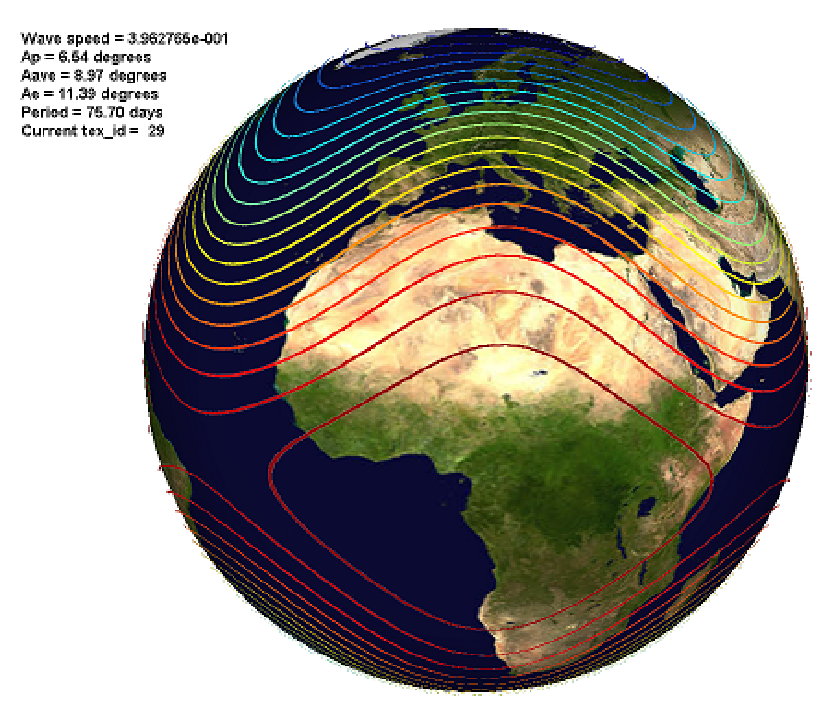
\includegraphics[scale=0.80]{viewer/view1.eps}
	\caption{Rossby-wave viewer output, Equatorial region}
	\label{fig:view1}
\end{figure}

A three-dimensional (3D) visualisation tool was developed to aid in interpreting the results, using the OpenGL 3D programming interface. The basic idea and aim was to be able to view progressive-wave free-surface contours superimposed on a rotating sphere in full 3D and real time. Additionally, it was required to translate these contours with respect to the rotating sphere so as to illustrate visually the propagation of the waves. OpenGL provides a convenient interface for accomplishing such a task, with built-in functions to handle the majority of the complex 3D calculations. We present here a brief overview of the processes utilised to implement this program (see, e.g., Hill~\cite{Hill:CGU} for an explanation of terms used in this discussion). The basic framework for the 3D program is loosely based around a tutorial on Jeff Molofee's OpenGL related website (see, http://nehe.gamedev.net); however substantial changes were required to implement the full program. Additionally, arc-ball camera movement in the program was implemented using Terence J. Grant's tutorial as a guide. This tutorial is also freely available on Jeff Molofee's website (see, http://nehe.gamedev.net/data/lessons/lesson.asp?lesson=48).

\begin{figure}[htbp]
	\centering
		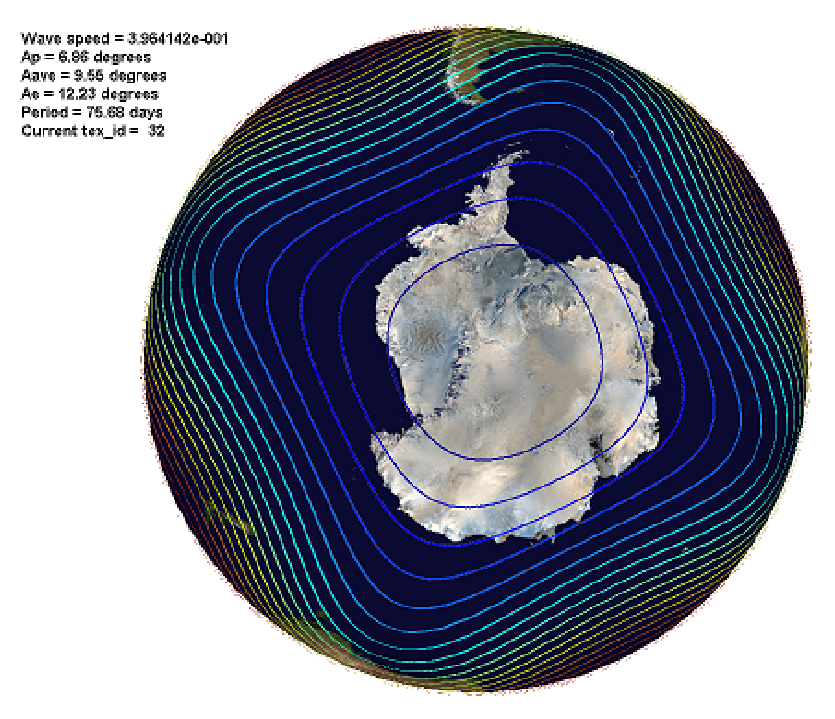
\includegraphics[scale=0.80]{viewer/view2.eps}
	\caption{Rossby-wave viewer output, Antarctic polar region}
	\label{fig:view2}
\end{figure} 

Full-colour free-surface contours were generated in MATLAB, for every point on each wavespeed-amplitude curve computed. These 2D images were then exported as encapsulated postscript files so they could be scaled without corruption. The images were then clipped and resized so as to be compatible with OpenGL texture loading. Because it was desirable to have a full-colour map of the Earth wrapped around the sphere, it was necessary to make only the contours in each image opaque, with the rest of the image being transparent so that the map of the Earth could be seen beneath the contours. For this reason, an alpha channel (transparency channel) was added to each image in order to let OpenGL know which parts of each contour image were visible; the alpha channel algorithm was written in MATLAB. The pictures were then saved using the PNG format, which supports the addition of an alpha channel.

Texture mapping (the process of mapping a 2D image onto a 3D surface) was used to load images of the Earth and free-surface contours, and then wrap each image around the surface of a sphere. Various rotations, which are standard functions of the OpenGL language, were then employed to translate the free-surface contours relative to the underlying image of the Earth. This gives the desired effect of the progressive waves moving relative to the fixed land beneath them. Readouts of the current progressive wavespeed, amplitude and period were placed in the upper left-hand corner of the screen, providing easy visual reference. 

\begin{figure}[htbp]
	\centering
		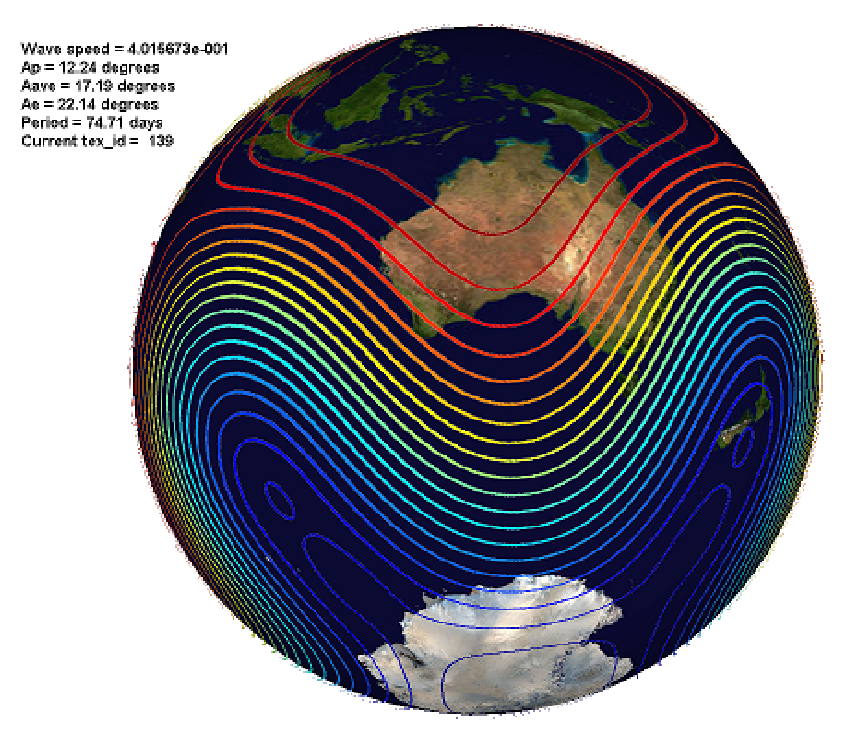
\includegraphics[scale=0.80]{viewer/view3.eps}
	\caption{Rossby-wave viewer output, Australian region}
	\label{fig:view3}
\end{figure} 

Additionally, a control mechanism was implemented to let a user step easily along the various computed solutions on each wavespeed--amplitude curve. In this manner, the transition and qualitative difference of solutions lying on different resonance branches is readily observed. Complete control over the viewing angle and zoom level were also implemented, providing visual access to any point on the globe with a simple click and drag or wheel scroll of the mouse. 

Figures~\ref{fig:view1}--\ref{fig:view3}, which are screen shots of the running program, illustrate the general output of the viewer, although it must be emphasised that the real program runs in full 3D and is interactive. The viewer has been designed to run on Windows 98/NT/2000/Me/XP operating systems, although a port to Linux would be possible, and requires a system with an OpenGL compliant graphics card with at least 32Mb of memory. The program and source code are freely available upon request to the author.